\documentclass[10pt]{article}
\usepackage{fullpage}
\usepackage{times}
\usepackage{amsmath,proof,amsthm,amssymb,color}
%\usepackage{multicol}
\usepackage{float}
\usepackage{graphicx}
\floatstyle{boxed} 
\restylefloat{figure}
\usepackage{hyperref}
\usepackage{listings}
%\usepackage[all]{hypcap}


\title{virtexsquared: ARM-like System-on-Chip on an FPGA}

\author{Joshua Wise\\
\texttt{$<$jwise@andrew.cmu.edu$>$} \and
Josiah Boning\\
\texttt{$<$jboning@andrew.cmu.edu$>$} \and
Bradley Yoo\\
\texttt{$<$bjy@andrew.cmu.edu$>$}}


\begin{document}
\maketitle

\begin{abstract}

The authors provide a report on the completed development of an ARM-like
System-on-Chip built on a Xilinx Virtex-5 FPGA.  A high-level overview of
the design is provided, as well as detailed examinations of various
submodules within the system.  

\end{abstract}

\vspace{0.1in} % fff fu LaTeX

\section{Introduction}

In fulfillment of the 18-545 Advanced Digital Design Capstone, this group
designed and implemented a peripheral layer for an ARM-like core. 
The system is built around two memory buses, and contains I/O cores to
interface with a smattering of peripherals, including:

\begin{itemize}
\item{DVI/VGA output from Chrontel CH7301C; video output is cached in a
framebuffer in main memory.}
\item{RS-232 serial output.}
\item{AC'97 audio with Analog AD1981B; audio output is cached in a
a simple main memory buffer.}
\item{PS/2 keyboard.}
\item{CompactFlash via the Xilinx SystemACE controller.}
\item{DDR2 SODIMM; interface glue is provided using Xilinx's predesigned
Memory Interface Generator (MIG) IP.}
\end{itemize}

The system contains various non-I/O cores to provide additional functionality,
including:

\begin{itemize}
\item{Timer}
\item{Bootstrap program preloader}
\item{Accelerators: memory set and image clear}
\end{itemize}

A primary goal of this peripheral layer is to be reused in 18-447; the system
is designed to be simple to interface with from a core perspective, and
hence usable for students in an introductory computer architecture class. 
The core, in particular, has a moderate \textit{anti}-goal of high
performance.

\part{Hardware Design}

\label{par:hardware}

In this part, we provide an overview of the design and implementation
decisions involved in the \textit{hardware} part of the system.  As a whole,
this section corresponds to the \texttt{rtl/} directory in the top level
source repository; the astute reader may follow along within.

\section{Memory Architecture}

\label{sec:memory}

The system, as a whole, is partitioned into two major access paths -- the
FSAB (\textit{Fast System Access Bus}), and the SPAM Bus (\textit{Slow
Peripheral Access Memory} Bus).  These two buses were designed to meet
wildly differing goals; the FSAB is designed for high-bandwidth, cachable
transactions, whereas the SPAMBus is designed for configuration space
register (CSR) accesses.  Ideally, most of the system's traffic will occur
over the FSAB.

\begin{figure}
  \centering
    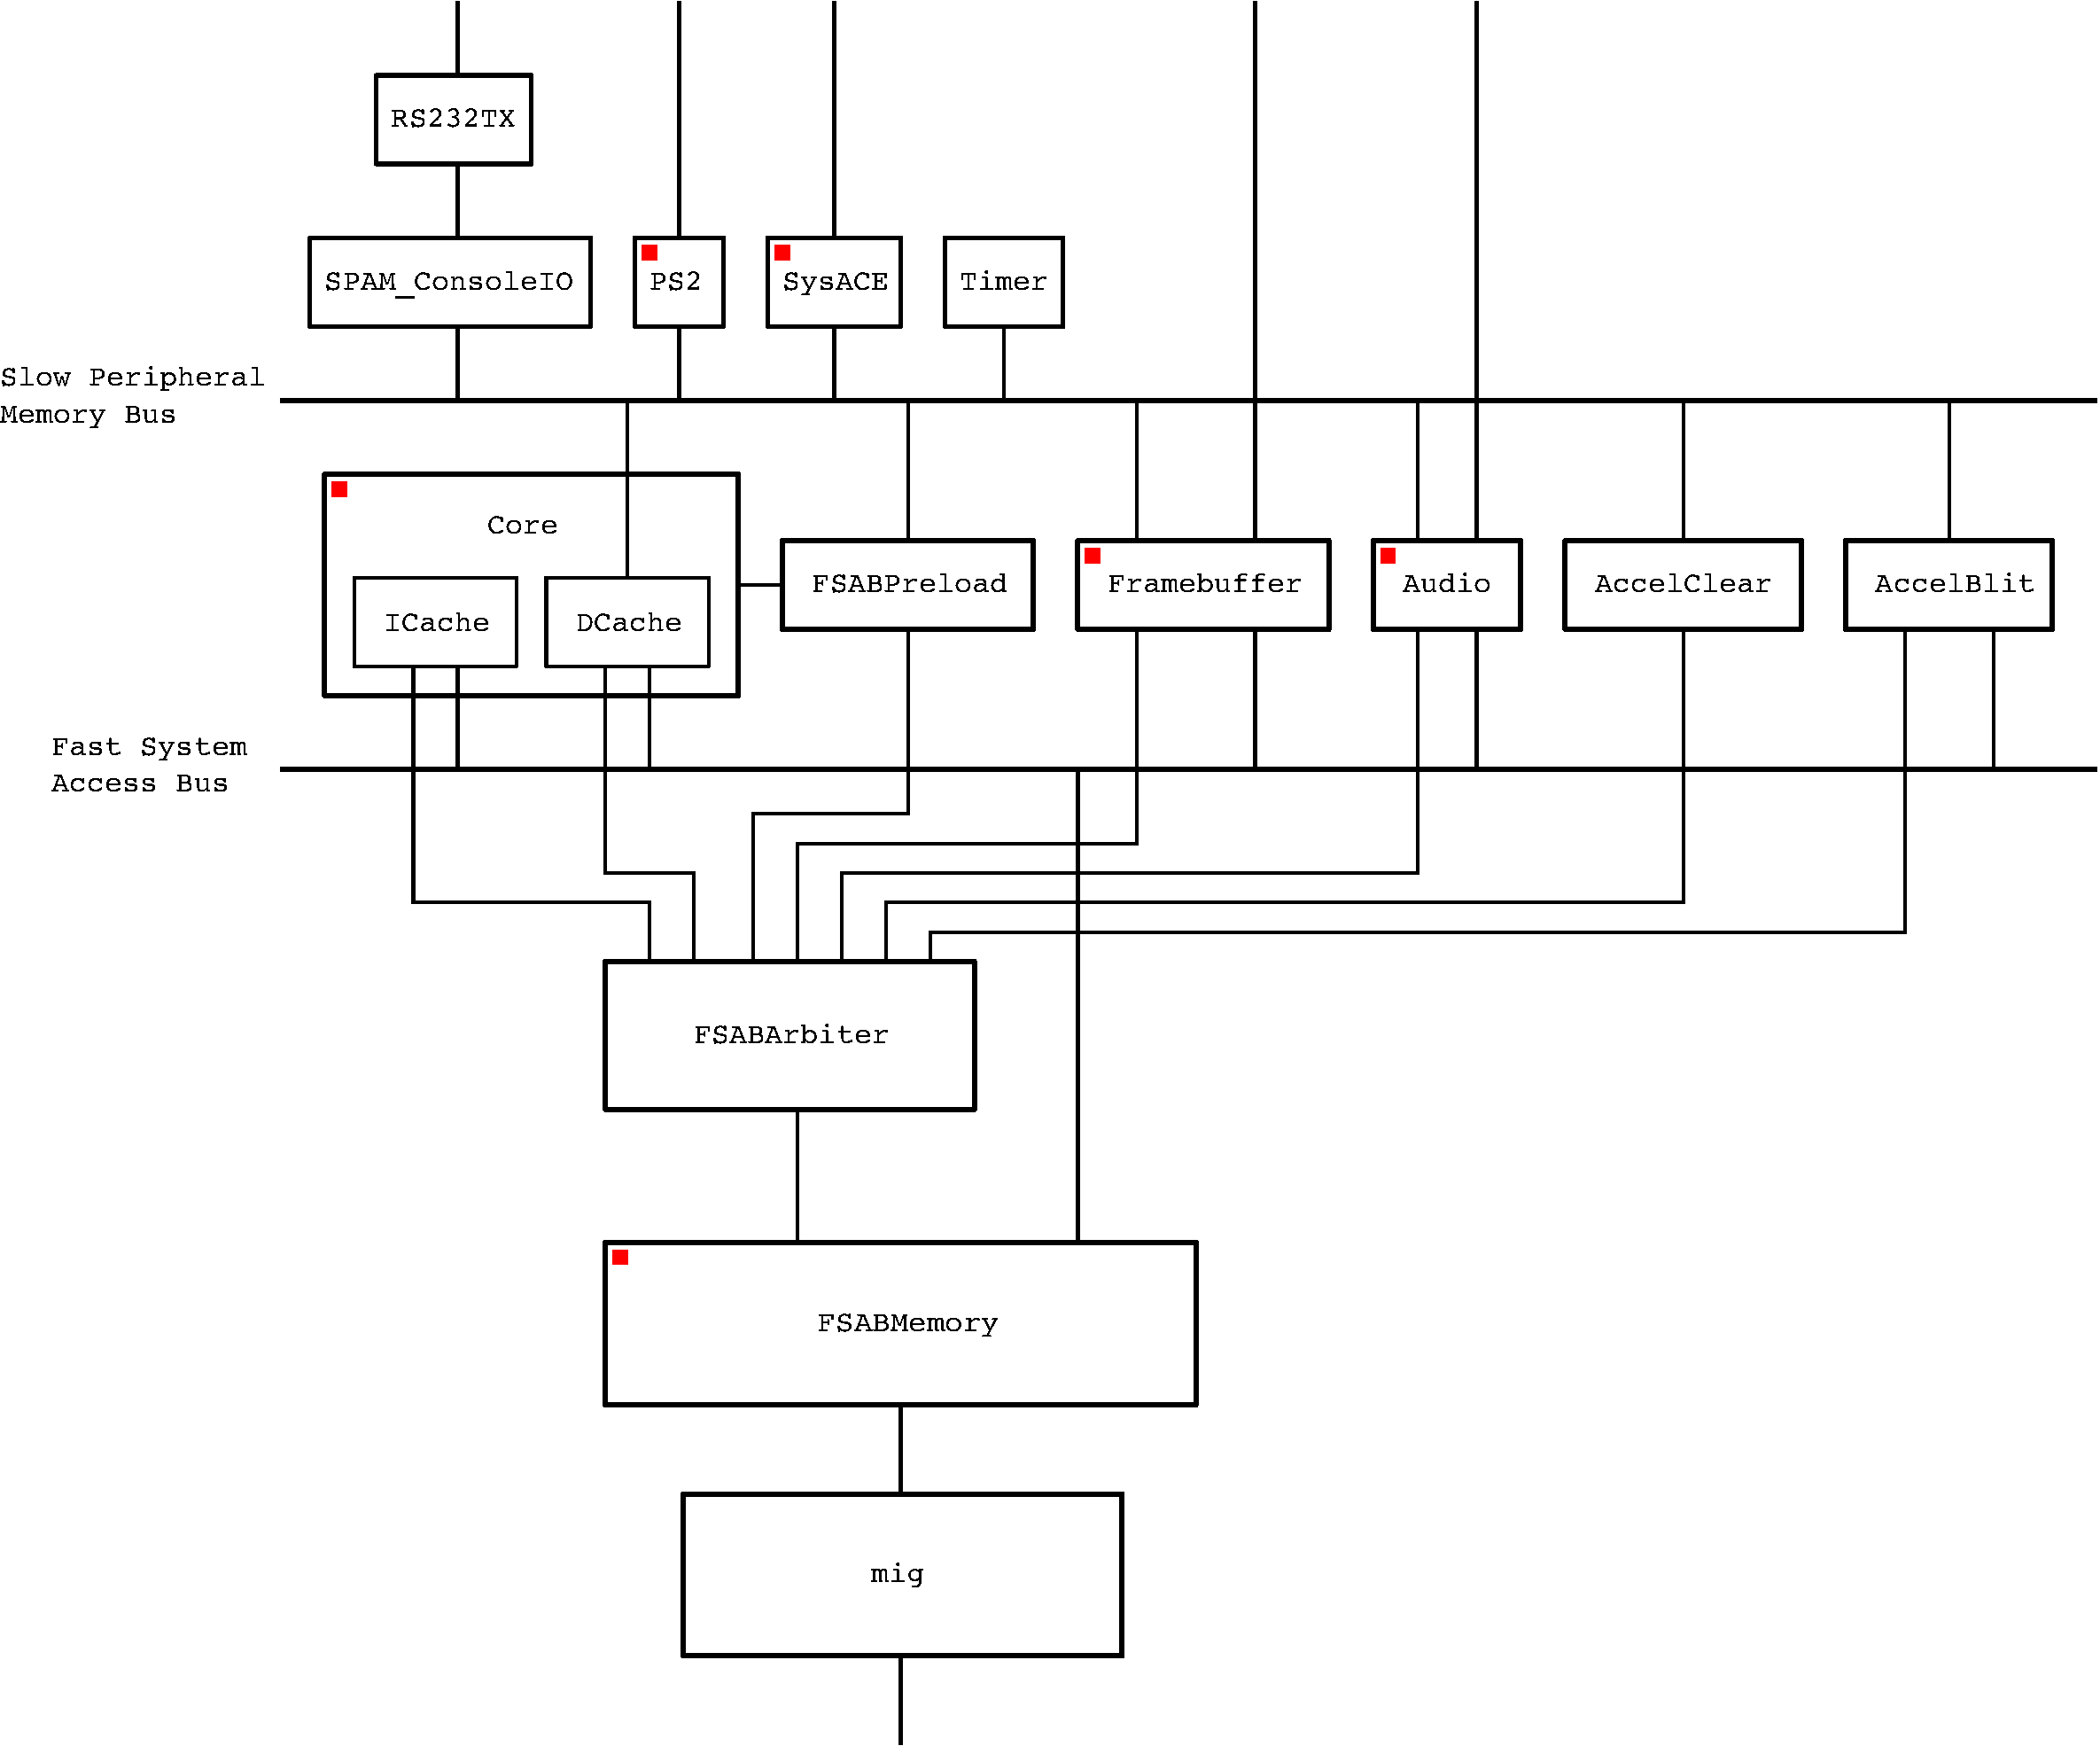
\includegraphics[width=.8\textwidth]{block_diagram.pdf}
  \caption{High-level system diagram. A red square in the corner of a module
           indicates a module where a ChipScope ILA is present and can easily
           be enabled.}
  \label{system_diagram}
\end{figure}

\subsection{Fast System Access Bus}

\label{sec:fsab}

The FSAB is a transaction-oriented bus designed primarily for accessing high-
latency memories such as DRAMs. The vast majority of the memory accesses on 
the system during normal operation (i.e., not at boot/ configuration time) 
will happen via the FSAB. 

\subsubsection{Terminology}

The FSAB works in terms of `transactions'. A read transaction shall consist 
of the `read request', and `read data' phases. A write transaction shall 
consist only of the `write data' phase.

Devices attached to the FSAB are classified as `masters' and `slaves'; a 
device that initiates transactions (reads and writes to main memory) is a 
master, and a device that completes transactions is a slave.

At times, it may be useful to discuss directions on the FSAB. For the purposes
of this discussion, data that is traveling from a master to a slave is 
considered `outbound' (and so signals for that purpose will begin with fsabo); 
similarly, data that initiates at the slave and returns to a master is 
considered `inbound' (and so signals for that purpose will begin with fsabi).


\subsubsection{Conceptual Overview}

virtexsquared, in its first incarnation, will only have a single memory 
controller. For that reason, the FSAB will be defined to have only one slave 
device - but since many peripherals may wish to do DMA access to or from main 
memory, the FSAB will be defined to potentially have many masters. The fact 
that only one slave device exists shall not be extensively exploited in either 
the design or implementation of the FSAB, since at a later time, a second 
memory controller may be interesting.

Since many memory controllers are capable of handling multiple pipelined 
requests, the FSAB supports multiple transactions in flight at a time. The 
slave will arbitrate these requests with a debit-credit system. Similarly, 
contention between masters will be resolved with an arbiter module that also 
performs queueing and debit-credit arbitration. In this regard, the bus 
arbiter should be ``invisible'' to a master; the debit-credit system should be 
interface-identical as if the master were talking directly to the slave.

Most operations that peripherals on the FSAB will perform will be in similar 
sizes. For instance, the I\$ and D\$ will always read sizes of a single cache 
line; the TLB will generally read page directory entries at a time; and the 
framebuffer will generally load half a FIFO's worth or so at a time. The 
general case, anyway, will not be a read of a single word. Similarly, writes 
will often be localized to each other. To facilitate this, each FSAB 
transaction will have a count of words up to a defined maximum of 8 along with 
the command and address. Inside each transaction, the address being written to 
shall autoincrement with each datum sent. Since not every datum may be 
interesting for a write, a ``write mask'' is also sent with every word written.

Since masters are isolated from each other by one or more arbiters, it is
generally not possible for one master to know what another master is doing.
Lacking any other form of cache coherency protocols (such as MOESI), a
system based around the FSAB is not cache-coherent! This means that the
applications programmer must take extra care to make sure that all data is
synchronized to main memory before allowing another peripheral to access
said data. (For instance, if the programmer wishes to write new data to the
frame buffer before flipping pages, he must cause the CPU to clean that
cache line by some mechanism first. In the current implementation, the data
cache is implemented as being write-through, so no such synchronization
issue takes place.)

The bus protocol is designed to be easy to implement by a DRAM-based slave. 
For that reason, the length of a read or write request is limited not just by 
the maximum, but by the alignment of the request. That is to say, if a request 
is only aligned to a four-qword boundary, but not to an eight-qword boundary, 
then the maximum size of the request is four qwords; a request of five or more 
qwords results in undefined behavior. (On the current DRAM-backed 
implementation, the resulting data comes from wrapping around the row buffer; 
on the current simulation-backed implementation, the resulting data comes from 
subsequent linear addresses.) 

\subsubsection{Design Overview: Portlist}

A FSAB master has the following ports outbound:

\begin{lstlisting}[basicstyle=\footnotesize,language=Verilog]
output                  fsabo_valid;
output [FSAB_REQ_HI:0]  fsabo_mode;
output [FSAB_DID_HI:0]  fsabo_did;
output [FSAB_DID_HI:0]  fsabo_subdid;
output [FSAB_ADDR_HI:0] fsabo_addr;
output [FSAB_LEN_HI:0]  fsabo_len;
output [FSAB_DATA_HI:0] fsabo_data;
output [FSAB_MASK_HI:0] fsabo_mask;
input                   fsabo_credit;
\end{lstlisting}

A FSAB master has the following ports inbound:

\begin{lstlisting}[basicstyle=\footnotesize,language=Verilog]
input                   fsabi_valid;
input  [FSAB_DID_HI:0]  fsabi_did;
input  [FSAB_DID_HI:0]  fsabi_subdid;
input  [FSAB_DATA_HI:0] fsabi_data;
\end{lstlisting}

No debit output (or input) is needed; a debit occurs implicitly when a new
FSAB transaction is begun. The credit input is always considered valid, even
if the inbound valid flag is not set.

\subsubsection{Design Overview: Transaction Specifics}

Transactions are defined by a start packet (and potentially additional data
packets) being sent to a slave, and the slave responding with any necessary
data packets. The slave may pipeline transactions as much as it is able
(credits can be returned before the slave has responded), but the slave
shall never reorder transactions. (Doing so would result in indeterminate
behavior with reads after writes, among other things.)

A start packet shall consist of the valid bit being set, the mode flag being
set to either FSAB\_READ or FSAB\_WRITE, the did/subdid set to the appropriate
values, an address, a length, and the first word of data and mask, should
they be valid for the current operation. Once a transaction is being sent
outbound, it shall not be interrupted by another transaction; the next data
packets are always part of this transaction. (For this reason, a master
should attempt to send packets as quickly as possible; excessive delay
between subsequent assertion of the valid flag may result in poor bus
performance.) In subsequent data packets, all control flags (i.e., all but
valid, data, and mask) are ignored.

The debit/credit system shall count each transaction as a debit, not each
word. Another transaction may be sent immediately after the credit flag is
asserted (or the credit may be queued).

The did field of each transaction shall be set as per each master's DID
assignment. The subdid may be set according to any internal state that the
master needs to track.

Some attention should be given to the mechanisms of clock distribution. In 
particular, it is permissible (and indeed often the case) that the inbound FSAB 
and outbound FSAB buses may be on different clock domains; usually the inbound 
FSAB clock comes directly from the slave, but the outbound FSAB clock is 
synchronous with the logic from the driving module. The outbound FSAB interface 
is then synchronized to the slave's clock in the arbiter. \footnote{This may be
considered a bug, as it departs from the conceptual goal that the bus arbiter 
is invisible to the master. From this perspective, it is preferable to have all
portions of the FSAB on the same clock domain, i.e. the slave's.}

\subsubsection{Known implementations}

The following are known implementations of the FSAB specification:

\begin{figure}
  \centering
    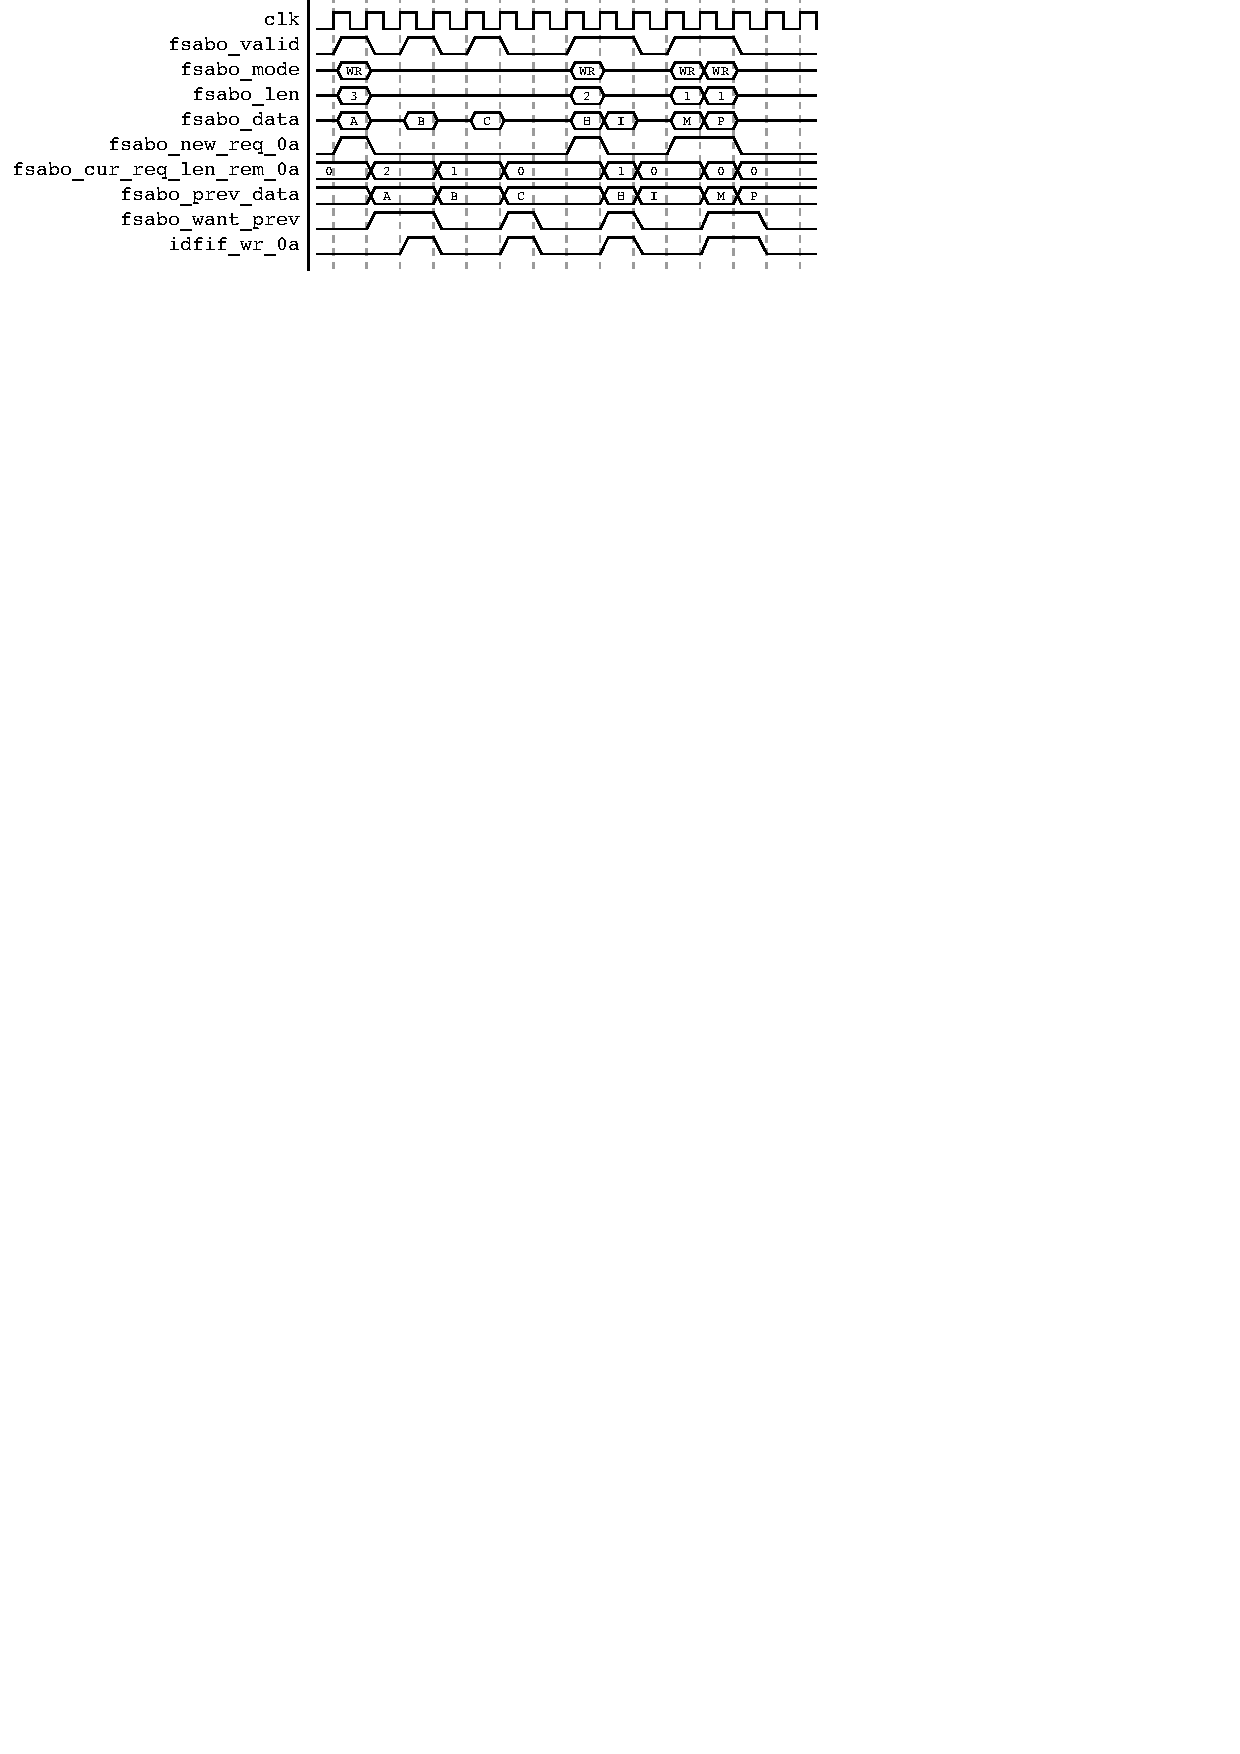
\includegraphics[width=0.85\textwidth]{FSAB-IxFIF.pdf}
  \caption{Clocking for memory controller.} \label{mshim_clock}
\end{figure}


\begin{itemize}
\item{Caches}
\item{Memory Controller}
\item{Arbiter}
\item{DMA Controller}
\end{itemize}

\subsection{Slow Peripheral Access Memory}
\label{sec:spam}

The SPAM bus is a word-oriented one-access-at-a-time bus designed primarily
for accessing configuration space registers (CSRs) on peripherals.

\subsubsection{Conceptual Overview}

In theory, all peripherals on the system will be matching and decoding on
the SPAM bus; when the processor does a SPAM-bus access, it is almost
certainly the case that a device will respond.  So, the bus should be
optimized for the common case in which a device responds shortly after a
request is sent.  Similarly, it should be the case that only one device ever
matches, so the bus need not be arbitrated between them; a simple OR'ing of
responses should work.

No peripheral should need to access any other peripheral's CSRs; any such
accesses from a debug interface should be multiplexed in between the CPU and
the SPAM-bus.  As such, the master-slave relationship in the SPAM-bus is
exactly the opposite of what it is on the FSAB; there is only one SPAM-bus
master, and there can be many SPAM-bus slaves.  Again, this property should
not be extensively exploited, but it is the case in the current
implementation.

Requests on the SPAM-bus should ordinarily be low latency, but there may be
need for wait states for various reasons.  For instance, if the other
peripheral is far away on the die, it may take an extra clock to compute the
appropriate response for a read.  A write, perhaps, may block until some
(short) action is complete.  There may also be a need to block because the
target peripheral is in a different clock domain, and a synchronizer needs
to shift the data over.

If no peripheral answers by deasserting busy\_b within a reasonable number
of cycles (usually 256), the request is deemed to have timed out, and a read
should return a value indicating that (usually something along the lines of
0xDEADDEAD).

\subsubsection{Design Overview: Portlist}

The processor has the following ports outbound:

\begin{lstlisting}[basicstyle=\footnotesize,language=Verilog]
output                  spamo_valid;
output                  spamo_r_nw;
output [SPAM_DID_HI:0]  spamo_did;
output [SPAM_ADDR_HI:0] spamo_addr;
output [SPAM_DATA_HI:0] spamo_data;
\end{lstlisting}

The processor has the following ports inbound:

\begin{lstlisting}[basicstyle=\footnotesize,language=Verilog]
input                   cio__spami_busy_b;
input  [SPAM_DATA_HI:0] cio__spami_data;
\end{lstlisting}

\subsubsection{Design Overview: Lifecycle of a request}

A request begins by the processor asserting the valid flag and specifying
the rest of the fields. This happens for exactly one cycle. Some time later
(potentially even on the same cycle), a device may assert the busy\_b flag
for one cycle to indicate that the request has been filled. Inbound data
shall be valid on the same cycle.

No new request shall be specified until either a previous request has returned, 
or a previous request has timed out. A request shall time out after no fewer 
than 128 cycles; the current DCache implementation times out after 256 cycles. 
When a device is not specifying data inbound, it shall drive its output port to 
zero; this allows the bus to simply OR together all responses.

Since the SPAM bus is always on the core's clock domain, some synchronization 
may be needed for CSRs on a different clock domain. Standard modules have been 
provided to synchronize reads and writes; for more information on those, see 
the documentation for the CSRAsync modules. 

\section{Core Microarchitecture}

As part of the virtexsquared system, the core must conform to the defined
bus protocols on the external interface (see section \ref{sec:memory}); but
within the core itself, anything goes.  Although the ARM core will not be
reused in future projects, the caches and global interface will be, and
hence potentially merit discussion.

\subsection{ARM Core}

The ARM core consists of the register file, fetch, decode, issue, execute,
memory, and the writeback units based off of Joshua's early FireARM core.
None of them are any good, and hence no more of them will be mentioned.

\subsection{Caches}
The caches each have a latency of one cycle. Upon missing, they send
requests for fills to the FSAB arbiter, which in turn propagates up to the
main memory. The caches have a zero-cycle latency for whether they have
missed; that is to say, the lookup takes place on the same cycle. In
addition to the standard FSAB connections, the Icache's port list is as
such:

\begin{lstlisting}[basicstyle=\footnotesize,language=Verilog]
input  [31:0] ic__rd_addr_0a;
input         ic__rd_req_0a;
output        ic__rd_wait_0a;
output [31:0] ic__rd_data_1a;
\end{lstlisting}

and the Dcache's port list is as such: (excluding SPAM and FSAB connections)

\begin{lstlisting}[basicstyle=\footnotesize,language=Verilog]
input  [31:0] dc__addr_3a;
input         dc__rd_req_3a;
input         dc__wr_req_3a;
output        dc__rw_wait_3a;
input  [31:0] dc__wr_data_3a;
output [31:0] dc__rd_data_4a;
\end{lstlisting}

The Icache and Dcache differ in two important ways. To wit:

\begin{itemize}
\item{The Icache is multi-way set associative. The number of ways is
controlled through a parameter. With the current Dcache architecture, this
is not feasible (due to the nature of writes).}
\item{The Dcache has a SPAM interface. The Icache cannot, because the SPAM
is single-master.}
\end{itemize}

Beyond these differences, though, the Icache and Dcache are very similar
internally. Both modules have two clock domains (the core clock and the FSAB
clock); data is received back inbound on the FSAB clock, and the core is
serviced on the core clock. Synchronization is performed internally in the
form of a read and write request service flag, similar to the internals of
the synchronizers.

\section{FSAB Internal Mechanisms}
\label{sec:fsabinternal}

Although the FSAB (described in the high level memory system overview; see
section \ref{sec:memory}) is conceptually simple, there are a few specific
portions of it that merit further explanation.  In particular, the system's
instruction cache is capable of reading only from the FSAB, leaving the
problem of how to bootstrap the system; and the FSAB specification makes no
mention of the mechanics of multiplexing multiple FSAB masters onto one bus. 
These issues are solved, respectively, by the FSAB Preloader and the FSAB
Arbiter.

\subsection{Preloader}
\label{sec:preloader}

In order to boot the system, instructions must first be somehow loaded into
memory, since the instruction cache is not capable of fetching from an
alternative non-volatile source. A few alternative options for this were
considered, and ultimately rejected. In brief, we considered:

\begin{itemize}
\item{adding an alternate path to the instruction cache during boot. This
was rejected, since it would add a potentially substantial amount of logic
to the critical path.}
\item{adding a SPAM interface to the instruction cache. This was rejected,
since the SPAM bus is not nominally capable of multi-master support, and
adding an arbitration mechanism would be necessary, which the protocol does
not easily support.}
\item{modifying the reset value for the instruction cache. This was rejected
since the code size available would be very limited, and support within
synthesis tools would be likely to be poor.}
\item{adding a second, non-volatile, slave to the FSAB. This was rejected
since the bus's architecture was mostly in place already, and a redesign to
support that would prove difficult in light of the requirement that
transactions return in order.}
\item{adding a preloader as an FSAB master. This was ultimately accepted.}
\end{itemize}

The preloader loads boot0, which is the first running software on the
system, into main memory.  (For more details about the boot sequence, see
section \ref{sec:boot}.) It acts as a simple FSAB master, with one
additional output - it has a mechanism to hold the CPU core in reset.  Since
it never does any reads, it has no fsabi interface; it only does size-8
writes to incrementing addresses.  Once DRAM has successfully been loaded,
the preloader has no function.  The data that it loads is stored in a ROM
that is implemented as a BRAM on an FPGA and as a simple ROM in simulation;
it is both synthesizable and simulatable.

The ROM for the preloader is compiled in from a \texttt{\$readmemh}
statement.  In synthesis, it is copied in during the build process (see
section \ref{sec:build}) from \texttt{sw/boot0/boot0.pad.hex64}; in
simulation, it is copied in from \texttt{tests/testbench.pad.hex64}.  These
are generated by a combination of \texttt{xxd} and \texttt{dd} during
software build.

\subsection{Arbiter}
\label{sec:arbiter}

Since the FSAB is a multimaster system, but the slave memory module has only
one master memory interface, there must be a multiplexing module to issue
requests in sequence to the slave memory.  In the system, this module is
called the FSABArbiter; it has a parameterizable number of fsabo ports as
inputs, and a single fsabo port as an output.  Given the debit/credit
system, not every request needs to be immediately dispatched to the slave
memory; indeed, each fsabo virtual-slave in the arbiter has a built in FIFO
(see section \ref{sec:fifo}) to buffer requests.

The buffer on the receiving end of each fsabo master also functions as a
clock domain synchronizer; by using the asynchronous FIFO, fsabo packets can
be safely transitioned from any system clock domain to the DRAM's clock
domain. Each buffer has, as a basic interface, a signal from the main
arbiter to begin outputting a transaction to the slave (if one is
available), and a signal to the main arbiter reporting completion of the
current transaction. (This may take zero cycles, if no transaction was
available, or it may take up to eight cycles, in the case of a
maximum-length write.)

The top-level arbiter makes no attempt at providing fairness between
peripherals.  The original goal was to include support for fairness, but it
was later discovered that doing so would require adding substantial logic to
the system, and potentially for \textit{negative} benefit; guaranteeing
bandwidth to the framebuffer and AC'97 proves to be invaluable in the face
of a high-bandwidth fill component that could potentially cause the
framebuffer's DMA engine to underrun.

\subsubsection{Interface}

Some mention should be given to the portlist, and how that is managed. Since
arrays of bitfields (i.e., two-dimensional bitfields) cannot be passed in
through a portlist in Verilog, all signals from the masters are concatenated
together into inputs of parameterized width. Internally, this looks somewhat
like this:

\begin{lstlisting}[basicstyle=\footnotesize,language=Verilog]
...
input [(FSAB_DEVICES*(FSAB_DATA_HI+1))-1:0]
      fsabo_datas;
...
\end{lstlisting}


Keeping all of the input signals synchronized and ordered, though,
especially in the face of the need for adding and removing new types of
modules quickly, sometimes proved difficult. To maintain our sanity in the
top-level module, we employed verilog-mode's \texttt{AUTOLISP} extensions along with
a small chunk of code provided to us by Michael Arntzenius. This prefixer
module is used as part of an \texttt{AUTO\_TEMPLATE}, as shown:

\begin{lstlisting}[basicstyle=\footnotesize,language=Verilog]
/*AUTO_LISP(setq list-of-prefixes '("pre" "fb"
            "audio" "ic" "dc" "accel_clear"))*/
...
/* FSABArbiter AUTO_TEMPLATE (
    ...
    .fsabo_valids(@"(template
        \"__fsabo_valid\")"),
    .fsabo_modes(@"(template
        \"__fsabo_mode[FSAB_REQ_HI:0]\")"),
    .fsabo_dids(@"(template
        \"__fsabo_did[FSAB_DID_HI:0]\")"),
\end{lstlisting}

When verilog-mode re-templates when \texttt{make auto} is run, all
instantiated ports in the arbiter will be automatically updated.  It is
important to note that the wire arrays \texttt{fsabo\_clks} and
\texttt{fsabo\_rst\_bs} must also be updated when a new device is added to the
\texttt{list-of-prefixes}; failing to do so will result in five hour long
debug sessions.  The arbiter assigns priority to incoming transactions based
on the order of the \texttt{list-of-prefixes}; that is to say, in the above
example, the preloader takes all available bandwidth before the framebuffer,
which takes remaining bandwidth before the AC'97 controller, etc.  The
screen-clear accelerator takes bandwidth \textit{last}, because it would otherwise
starve the rest of the system for bandwidth.

\section{Memory Controller}

In the virtexsquared memory system (see section \ref{sec:memory}), the
memory controller is the sole client on the FSAB.  The memory controller
acts as an intermediary between the FSAB and the coregen-produced Memory
Interface Generator (MIG).

\subsection{Interfaces}

On the side facing the FSAB and the rest of the virtexsquared system, the
memory controller behaves as a slave as specified in the FSAB specification
(see section \ref{sec:fsab}).

On the side facing the MIG, the memory controller behaves as specified in
the Xilinx Memory Interface Generator documentation.

\subsection{Implementation}

\begin{figure}
  \centering
    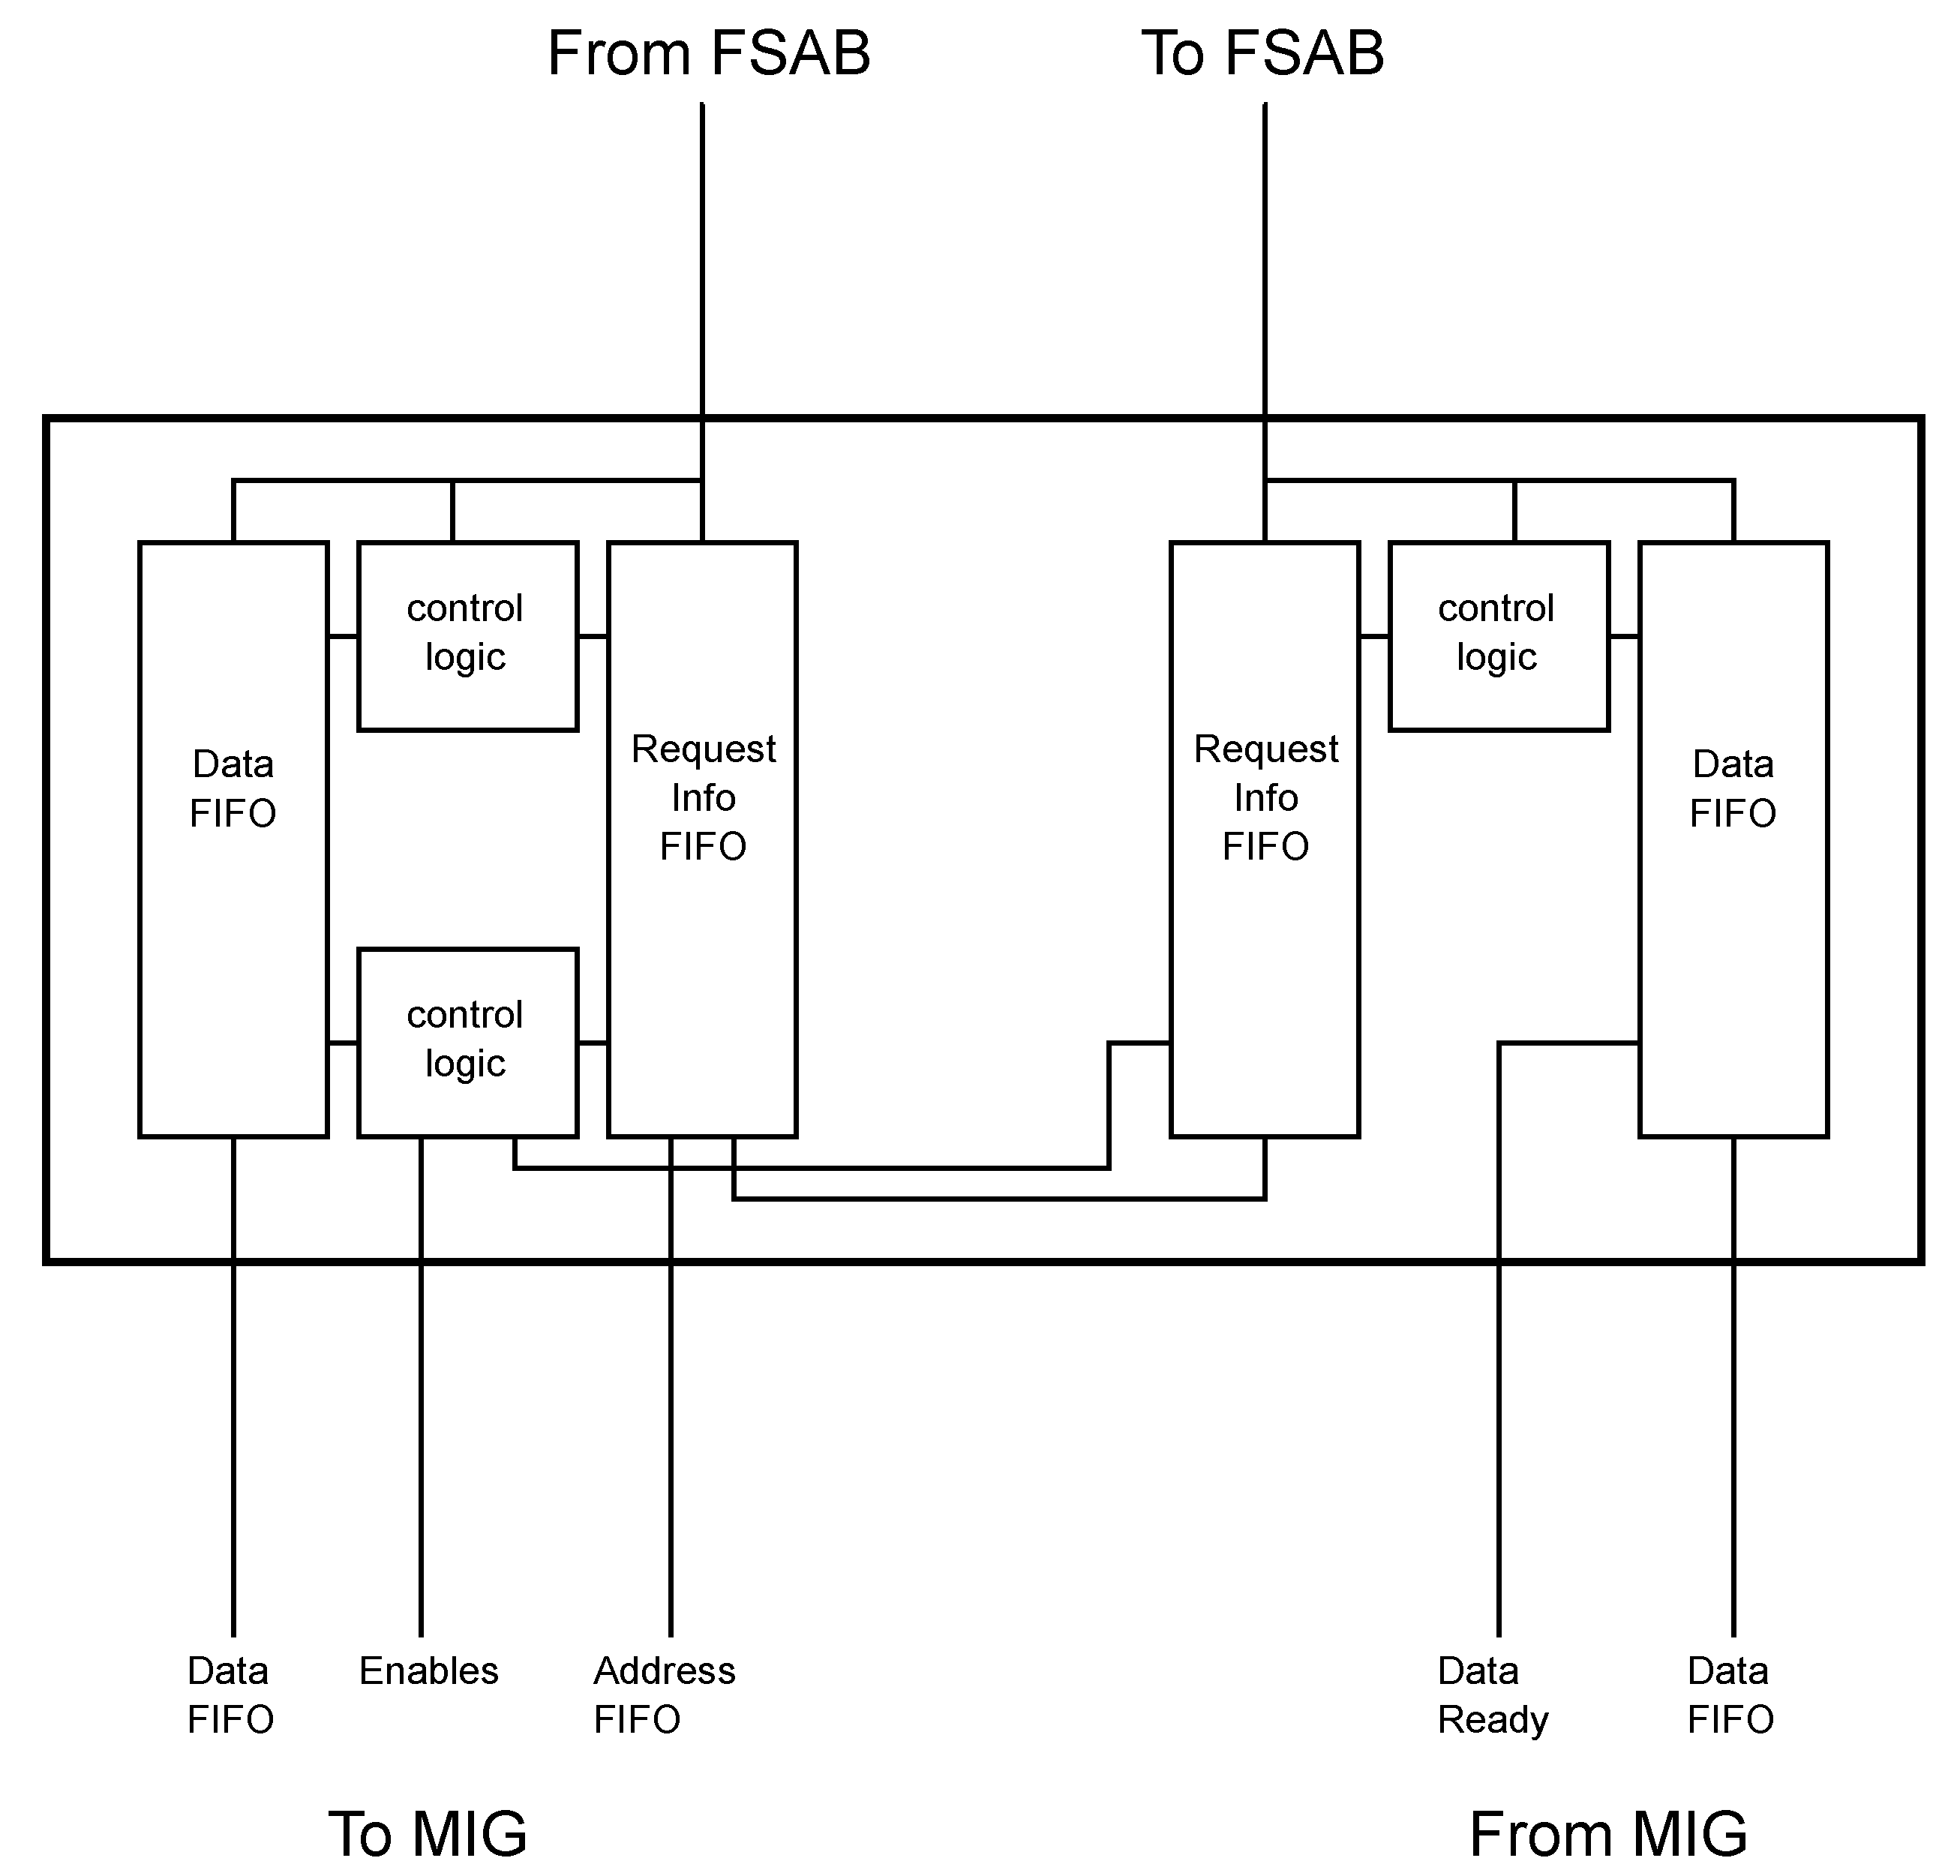
\includegraphics[width=0.85\textwidth]{FSABMemory.pdf}
  \caption{Internals of the memory controller.} \label{fig:fsabmemory}
\end{figure}


The memory controller is best described by tracing the lifetime of a request
as it is made on the FSAB, passes through the memory controller and MIG, and
is returned to the requesting device. At the first packet of the request,
the device identifiers, address, and length are stored in the request info
FIFO. If the request is a write request, the controller reads packets of
data into the data FIFO until the entire request is stored in the FIFO. Each
entry in the data FIFO is two packets wide; the MIG requires data to be
double-wide to facilitate DDR memory. If a write request is not aligned, the
controller inserts a packet's worth of masked data at the front of the
request.

Once the entire transaction has been stored in the FIFOs, the controller
sends it to the MIG. The MIG performs burst operations of a standard length
(in the current implementation, 8 words of 64 bits each; because the memory
is DDR, it takes four clock cycles to transmit or receive a burst). The
request begins with a write to the MIG address and command FIFOs. On a write
request, the first write to the data and mask FIFOs is in the same clock
cycle, and the rest of the burst follows on consecutive cycles. If the
actual request is shorter than the burst length, masked data is written for
the remainder of the burst. On a read request, the device identifier and
request length are stored in the output request info FIFO.

On a read request, some time after sending the request to the MIG, the MIG
will send data back. This data is read into the output data FIFO. When the
data FIFO becomes not empty, the controller reads the device identifier and
length from the request FIFO and the first row from the data FIFO. Data is
returned to the device, with reads from the double-width FIFO every two
packets, until the full length has been transmitted.

\subsection{Known Bugs}

\begin{itemize}
\item{Reads not aligned to whatever boundary the MIG wants are incorrect
(the address is not stored in the output-side request info FIFO, so the
output side has no way to know that the first data the MIG returns is not
the requested data).}
\item{Reads not of the full burst length may mess everything up, since I
don't think we discard the rest of the data the MIG returns in its burst.}
\end{itemize}

\section{Simple DMA Read Controller}
\label{sec:dmac}

The Simple DMA (Direct Memory Access) Read Controller provides a FIFO-like
interface for a target peripheral to read from memory.

\subsection{Motivation}

Since many devices require memory read access in a linear pattern, it only
made sense to support such access pattern in a simple way.

\subsection{Conceptual Overview}

After providing a start address, length, and a trigger command through the
SPAM bus (see section \ref{sec:spam}), data\_ready will be asserted high and
the master will be able to get the next 8 bytes of data one cycle after
request is asserted high as long as the FIFO (queue) is not empty (no
underflow).  Once the DMA is done reading through the entire length, it may
be triggered again to read from a new start address and different length.

\subsection{Design Overview}

\subsubsection{Portlist}

Simple DMA Read Controller has the following ports that the master should
not directly interact with:

\begin{itemize}
\item{the default FSAB portlist (prefixed by dmac\_\_ for outbound)}
\item{SPAM portlist (prefixed by dmac\_\_)}
\end{itemize}

For the master, it has the following ports:

\begin{lstlisting}[basicstyle=\footnotesize,language=Verilog]
input request; 
input target_clk; /* clk that the master is running in */
input target_rst_b;
output [63:0] data; /* 8 bytes of new data */
output data_ready;
output fifo_empty; 
/* asserted when the fifo is empty. This may be the case when there is an
 * underflow or when the DMA didn't start reading */
\end{lstlisting}

\subsubsection{Parameters}

\begin{lstlisting}[basicstyle=\footnotesize,language=Verilog]
parameter FIFO_DEPTH = 128; /* must be a power of 2 */
parameter FIFO_HI = clog2(FIFO_DEPTH) - 2;
parameter FSAB_DID = 4'hF;
parameter FSAB_SUBDID = 4'hF;
parameter SPAM_DID = 4'hx;
parameter SPAM_ADDRPFX = 24'h000000;
parameter SPAM_ADDRMASK = 24'hFFFFE0;
parameter DEFAULT_ADDR = 31'h00000000;
parameter DEFAULT_LEN = 31'h00000000;
\end{lstlisting}

The parameters are defined as follows:

\begin{itemize}
\item{\textbf{FIFO\_DEPTH}: Depth of the internal FIFO. DMA Controller will
try to keep this FIFO as full as possible. This value must be a power of 2
and 8 or greater to be functional.}
\item{\textbf{FIFO\_HI}: Highest bit needed to represent FIFO\_DEPTH space.
(log${}_2$(FIFO\_DEPTH) - 2) if FIFO\_DEPTH is power of 2.}
\item{\textbf{FSAB\_DID}: FSAB device id of the master. (if the master
doesn't have one, give the master one by setting it in
\texttt{rtl/fsab/fsab\_defines.vh})}
\item{\textbf{FSAB\_SUBDID}: FSAB sub device id of the master. (if the
master doesn't have one, give the master one by setting it in
\texttt{rtl/fsab/fsab\_defines.vh})}
\item{\textbf{SPAM\_DID}: SPAM device id of the master. (if the master
doesn't have one, give the master one by setting it in
\texttt{rtl/spam/spam\_defines.vh})}

\item{\textbf{SPAM\_ADDRPFX} and \textbf{SPAM\_ADDRMASK}: To write/read from
the SPAM bus, it must be the case that \texttt{((spamo\_addr \& SPAM\_ADDRMASK) ==
SPAM\_ADDRPFX)}.  (Note: Always set the last 5 bits of the SPAM\_ADDRMASK to
0.)}

\item{\textbf{DEFAULT\_ADDR}: Default starting address for the DMA.}

\item{\textbf{DEFAULT\_LEN}: Default length that the DMA will read. The DMA will
provide values starting from address up to the length.}

\end{itemize}

\subsubsection{Config Registers (SPAM)}

The following values come from \texttt{rtl/fsab/dma\_config\_defines.vh};
these addresses correspond to the last 5 bits that the spamo\_addr needs to
be set to refer to these registers.

\begin{lstlisting}[basicstyle=\footnotesize,language=Verilog]
parameter NEXT_START_REG_ADDR = 5'h000;
parameter NEXT_LEN_REG_ADDR = 5'h004;
parameter COMMAND_REG_ADDR = 5'h008;
parameter FIFO_BYTES_READ_REG_ADDR = 5'h00c;
parameter TOTAL_BYTES_DELIVERED_REG_ADDR = 5'h010;
parameter CURR_START_REG_ADDR = 5'h014; 

parameter DMA_STOP = 2'b00;
parameter DMA_TRIGGER_ONCE = 2'b01;
parameter DMA_AUTOTRIGGER = 2'b10;
\end{lstlisting}

The registers are defined as follows:

\begin{itemize}
\item{\textbf{NEXT\_START\_REG (write only)}: sets the starting address of
the DMA for the \textbf{next time} it is triggered.}

\item{\textbf{NEXT\_LEN\_REG (write only)}: sets the length that the DMA has
to read for the \textbf{next time} it is triggered.}

\item{\textbf{COMMAND\_REG (write only)}: sets the next command for the DMA
engine to execute, from one of:}
\begin{itemize}
\item{\textbf{DMA\_STOP}: DMA does not trigger again.}
\item{\textbf{DMA\_TRIGGER\_ONCE}: Triggers the DMA once.}
\item{\textbf{DMA\_AUTOTRIGGER}: Everytime, the DMA is done reading, it is
triggered again.}
\end{itemize}

\item{\textbf{FIFO\_BYTES\_READ\_REG (read only)}: the number of bytes that
the \textit{internal FIFO} has read so far since it was last triggered.}

\item{\textbf{TOTAL\_BYTES\_DELIVERED\_REG (read only)}: the total number of
bytes that was delivered to the master since the \textit{last reset}. (note:
it is not ``last triggered'')}

\item{\textbf{CURR\_START\_REG (read only)}: the address that the DMA
started reading from. (It provides the value of NEXT\_START\_REG before it was
triggered)}

\end{itemize}

\subsubsection{Implementation}

The internal queue for DMA is represented in the following way:

\begin{lstlisting}[basicstyle=\footnotesize,language=Verilog]
reg [FSAB_DATA_HI:0] fifo [(FIFO_DEPTH-1):0];
 
/* Clock domain: fsabi_clk */
reg [FIFO_HI:0] fifo_wpos;
 
/* Clock domain: target_clk */
reg [FIFO_HI+1:0] curr_fifo_length;
reg [FIFO_HI:0] fifo_rpos;
\end{lstlisting}

While the DMA is triggered, it attempts to obtain data in 64 byte blocks
using FSAB as long as there is space in the queue for it. When the request
for 64 byte block is sent, these data will come 8 bytes at a time. Whenever,
a value arrives, the value is stored in the fifo but \textbf{only} fifo\_wpos changes
values. Once all 64 bytes arrive, a completion message gets synchronized
from fsabi\_clk domain to target\_clk domain so that curr\_fifo\_length can be
updated. fifo\_rpos is used to read values from the fifo to provide data to
the master.

\subsection{Users}

The Simple DMA Read Controller is used by:

\begin{itemize}
\item{Framebuffer (see section \ref{sec:framebuffer})}
\item{Audio (see section \ref{sec:audio})}
\end{itemize}

\section{Framebuffer}
\label{sec:framebuffer}

The framebuffer provides pixeldata to the DVI to be displayed on the screen.

\subsection{Conceptual Overview}

Framebuffer uses the Simple DMA Read Controller (see section \ref{sec:dmac})
to obtain pixel data to be displayed and uses SyncGen to figure out whether
the value needs to be sent for display.

Notes:

\begin{itemize}
\item{Four bytes contain data for one pixel.}
\item{Each primary color uses one byte (RGB) and occupies the first 3
bytes.}
\item{The last byte is thrown away.}
\item{(Be aware of little endianness while programming...)}
\end{itemize}

\subsection{Framebuffer DMA configuration}

These can be accessed through 0x820000$<$Register Addr$>$

Some relevant addresses for the framebuffer are:

\begin{itemize}
\item{\textbf{0x82000000 (write only)}: Framebuffer DMA start address (for setting buffer
locations)}
\item{\textbf{0x82000004}: Framebuffer length}
\item{\textbf{0x82000014 (read only)}: Start address of the buffer currently being read by
the DMA (needed for triple buffering).}
\end{itemize}

\subsection{Example Usage}

The Framebuffer is used by the multibuf library (see section
\ref{sec:multibuf}).



\section{Peripheral Architecture}

is another section to be filled in.

\part{Software Design}

In this part, we mention salient libraries that we designed to abstract some
of the details of the hardware.

\part{Miscellaneous System Notes}

In this part, we describe other portions of the system that do not easily
fit as being called either hardware or software, but that still merit
discussion.

\section{virtexsquared Boot Sequence}
\label{sec:boot}

Since the sequence of steps that virtexsquared takes to boot is somewhat
unlike a modern x86 PC, it is worth discussing in brief. Specifically, in
order to boot, control of the system first starts with the SystemACE, is
passed to the preloader, then to boot0, then boot1, and then finally to
application code.

\subsection{SystemACE}

When the board is first powered on, there is no configuration loaded on the
FPGA. In order to get the virtexsquared system running at all, the
configuration must be somehow loaded. If the CompactFlash card is inserted
(and contains the BOOT.ACE file generated from the bitstream), then the
Xilinx SystemACE CompactFlash controller on the board will begin programming
the FPGA over the configuration JTAG interface; this procedure takes about a
second and a half. If CompactFlash FPGA programming fails, then the red LED
on the board will either blink or illuminate statically.

The SystemACE can also be removed from this stage of boot by programming the
board using the external JTAG connector; this is useful when debugging the
design using ChipScope.

When the FPGA is programmed, the internal circuitry begins a post-reset
sequence.

\subsection{Preloader}

Once the FPGA has been configured, the PLLs and DCMs have locked, and the
DRAM PHY has self-calibrated, the preloader is taken out of reset, and
begins performing DMA from an internal block RAM into the very beginning of
DRAM (address 0x0). The preloader DMAs in 8-qword blocks, and transfers a
total of 16 kBytes of data into DRAM. While this occurs, the core is held in
reset using a signal OR'ed in with the normal reset path.

Once the preloader completes, the core is taken out of reset and allowed to
begin operating.

The operation and design behind the preloader is discussed in more detail in
section \ref{sec:preloader}.

\subsection{boot0}

boot0 is the first code that is executed by the ARM core. It begins with a
small fragment of ARM assembly, called \texttt{crt0}, which sets up a stack
pointer, and zeroes the \texttt{.bss} section.  Once it has done those, the
C runtime environment is ready, and \texttt{crt0} jumps into the main
function.  The main function prints some text to the console, initializes
the SystemACE's microprocessor interface, paints the boot display, and loads
and jumps to boot1.

Importantly, boot0 does not know anything about any executable formats, and
it does not know anything about filesystems; the limitation of its
intelligence is in finding a partition that is marked as bootable, and
loading the first 512 kBytes of that partition to a specific address in
memory (0x4000). If any sector read fails, then boot is aborted; if the
partition cannot be found, or the CompactFlash is not present, then boot is
also aborted. boot0 has a minimum feature set because it is baked into the
preloader's Block RAM; making changes to boot0 costs 20 minutes to recompile
the core, and so it is of the utmost import that boot0 be solid, versatile,
and stable.

If boot is aborted, or the boot1 program returns control to boot0, then the
message ``\texttt{Control returned to boot0; press reset to retry boot}'' will
be printed to the serial console, and the colorbars and color-cycling
virtexsquared logo are displayed on screen.  (See figure \ref{img:boot0}.)

\begin{figure}
  \centering
    
\includegraphics[width=0.49\textwidth]{boot0.png}
  \caption{boot0's failure display.} \label{img:boot0}
\end{figure}

\subsection{boot1}

boot1 is the next stage of code executed by the ARM core. It, too, begins
with a \texttt{crt0}, but this \texttt{crt0} does not need to set up the
stack pointer; all future stack usage on the system will be on the same
stack as that set up by boot0.  The main differences from boot0 to boot1
are:

\begin{itemize}
\item{boot1 does not paint a splash screen. The system has already been
shown to be "alive" by boot0; boot1 needs to take no further steps in that
regard.}
\item{boot1 is capable of reading the FAT16 partition on the CompactFlash.
boot0 does not have this capability, since boot0's feature set must be
small.}
\item{boot1 is capable of loading an ELF file. boot0 loads a flat memory
image, as created by \texttt{objcopy}; boot1 loads full ELF programs that
may have many segments.}
\item{boot1 is replaceable with a minimum of pain by \texttt{dd}'ing over a
partition; boot0 requires a resynthesis to replace.}
\end{itemize}

When boot1 takes control of the system, it first initializes the SystemACE,
and then mounts the FAT16 partition. It then prints the contents of the root
directory to the serial console. If GAME.ELF exists on the partition, boot1
loads it into memory at 0x01000000 (+16MB), and then hands the loaded image
off to the ELF loader. If all of the above succeed, boot1 prints a message
indicating that it is transferring control to the application code, and then
jumps to the game's entry point.

If boot1 fails, it may emit any of a few diagnostics. The message
``\texttt{boot1 exiting}'' indicates that for some reason, boot1 completed
and is returning control to boot0.  The message ``\texttt{ELF loading
failed}'' indicates that boot1's ELF loader determined that the file format
was invalid for some reason; common causes are a flash card that has not
been properly unmounted, and hence had become corrupted.

\subsection{Application}

Once boot1 has loaded GAME.ELF from the CompactFlash card, the application
is running. The initialization sequence of the application code involves
loading a series of resources and eventually presenting a menu.

\section{Tools}

virtexsquared is developed using some standard tools, and some custom tools. 
The parts of the virtexsquared development system that appared to be of
particular use are elucidated below.

\subsection{Xilinx XST}

\subsection{verilog-mode}

\subsection{GNU make}

\subsection{makecdc for ChipScope}

\subsection{j4cbo}

\subsection{git}

\part{Project Logistics}

In this part, we describe the logistics of the completion of this project,
including miscellaneous sections required for completion of this report.

\section{Schedule}

Gantt chart is figure 3.  We are behind it.  I ran out of time to write
this because I spent all night debugging.

\begin{figure*}
  \centering
    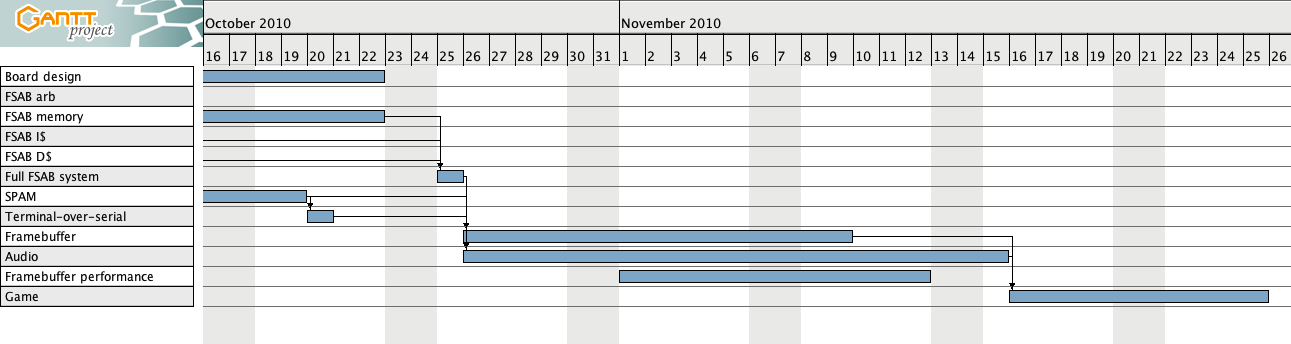
\includegraphics[width=\textwidth]{gantt-chart.png}
  \caption{I hate Xilinx.} \label{mshim_clock}
\end{figure*}

\end{document}
